\chapter{Optimal Control and Non-Linear Optimization Basics\label{chapter:optimization}}

\ifpdf
    \graphicspath{{ChapterOptimizationIntroduction/figures/Raster/}{ChapterOptimizationIntroduction/figures/PDF/}{ChapterOptimizationIntroduction/figures/}}
\else
    \graphicspath{{ChapterOptimizationIntroduction/figures/Vector/}{ChapterOptimizationIntroduction/figures/}}
\fi

In previous chapters, we investigated the tools for modeling a floating base system that establishes a set of contacts with the environment. This chapter introduces the basics and terminology of \emph{non-linear programming} and \emph{optimal control}. We then take advantage of the technique presented here to design the controllers analyzed in Part~\ref{part:wbc} and Part~\ref{part:simplified}.
Non-linear programming is the mathematical process of finding a set of variables such that a non-linear function is minimized (or maximized). Once the theory of \emph{non-linear programming} is introduced, we apply it to the resolution of the \emph{optimal control} problems. 
The \emph{optimal control theory} is a branch of control theory that aims at finding a control for a dynamic system over a period of time such that an objective function is optimized.
\par
The chapter will take an \emph{utilitaristic} approach to describe such frameworks, to this concern we decided to avoid focusing on the rigorous proofs. The reader who wants a more rigorous understanding of non-linear optimization theory should consult the extensive literature. Here, it is worth mentioning \citep{Boyd2004ConvexOptimization,Chachuat2007NonlinearPractice,diehl2009efficient} from which parts of this chapter took inspiration. On the other hand, complete and rigorous manuscripts on optimal control are \citep{Boyd2004ConvexOptimization,bemporad2002hybrid,Qin2000AnApplications,Biral2016NotesProblems,Allgower1999NonlinearOverview}.
\par
The chapter is organized as follows.
Sections~\ref{sec:convex_set} and~\ref{sec:convex_function} give an overview of convex sets and convex functions, respectively. Section~\ref{sec:optionization_problem} introduces the optimization problem. Section~\ref{sec:qp} presents the Quadratic Programming problem as a special case of the optimization problem. The Quadratic Programming problem will be extensively exploited in the design of the whole-body controllers presented in Part~\ref{part:wbc}.  Section~\ref{sec:optimal_control} and \ref{sec:mpc} introduce some of the basics of Optimal Control and Model Predictive Control. The content of Section~\ref{sec:mpc} will be crucial to fully comprehend the design of the controllers detailed in Part~\ref{part:simplified}.




\tikzset{every picture/.style={line width=0.75pt}} %

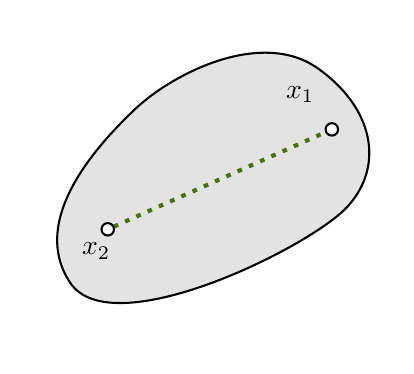
\begin{tikzpicture}[x=0.75pt,y=0.75pt,yscale=-1,xscale=1]

\draw  [fill={rgb, 255:red, 227; green, 227; blue, 227 }  ,fill opacity=1 ] (147.67,149) .. controls (166.24,131.29) and (208.86,110) .. (235.86,129) .. controls (262.86,148) and (268.33,175.95) .. (250.33,195.67) .. controls (232.33,215.38) and (136.71,262.43) .. (116.71,232.43) .. controls (96.71,202.43) and (129.1,166.71) .. (147.67,149) -- cycle ;
\draw [color={rgb, 255:red, 65; green, 117; blue, 5 }  ,draw opacity=1 ][line width=1.5]  [dash pattern={on 1.69pt off 2.76pt}]  (242.75,158.5) -- (134.79,206.64) ;
\draw  [fill={rgb, 255:red, 255; green, 255; blue, 255 }  ,fill opacity=1 ] (239.75,158.5) .. controls (239.75,156.84) and (241.09,155.5) .. (242.75,155.5) .. controls (244.41,155.5) and (245.75,156.84) .. (245.75,158.5) .. controls (245.75,160.16) and (244.41,161.5) .. (242.75,161.5) .. controls (241.09,161.5) and (239.75,160.16) .. (239.75,158.5) -- cycle ;
\draw  [fill={rgb, 255:red, 255; green, 255; blue, 255 }  ,fill opacity=1 ] (131.79,206.64) .. controls (131.79,204.99) and (133.13,203.64) .. (134.79,203.64) .. controls (136.44,203.64) and (137.79,204.99) .. (137.79,206.64) .. controls (137.79,208.3) and (136.44,209.64) .. (134.79,209.64) .. controls (133.13,209.64) and (131.79,208.3) .. (131.79,206.64) -- cycle ;

\draw (120.89,211.72) node [anchor=north west][inner sep=0.75pt]    {$x_{2}$};
\draw (219.25,136.44) node [anchor=north west][inner sep=0.75pt]    {$x_{1}$};


\end{tikzpicture}
\section{Convex function\label{sec:convex_function}}
Given a function $f: \mathbb{R}^n \rightarrow \mathbb{R}$, we say that $f$ is \emph{convex} if
\begin{enumerate}
    \item the domain of $f$, denoted with $\dom(f)$ is a convex set;
    \item for all $x_1,x_2 \in \dom(f)$  and $0 \le \theta \le 1$ we have 
    \begin{equation}
        f(\theta x_1 + ( 1- \theta) x_2) \le \theta f(x_1) + (1-\theta) f(x_2).
    \end{equation}
\end{enumerate}
To give the reader a better understanding, we can imagine drawing a chord from any $x_1$ to $y_1$, if it lies above the graph of $f$, $f$ is convex.
A function $f$ is \emph{strictly convex}, if for $x_1 \ne x_2$ and $0<\theta<1$, we have $f(\theta x_1 + ( 1- \theta) x_2) < \theta f(x_1) + (1-\theta) f(x_2)$. If $-f$ is (strictly) convex, then $f$ is said to be (strictly) concave. Figure~\ref{fig:convex_nonconvex_functions} illustrates an example of convex and nonconvex functions.

\begin{figure}[t]
\centering
    \begin{subfigure}[b]{0.48\textwidth}
        \centering
        \includegraphics{chapter_optimization_introduction/figures/first-order_condition_convex_function.tikz}
        \caption{Convex function.}
        \label{fig:first-order_condition_convex_function}
    \end{subfigure}
    \hfill
    \begin{subfigure}[b]{0.48\textwidth}
        \centering
        \includegraphics{chapter_optimization_introduction/figures/nonconvex_function.tikz}
        \caption{Nonconvex function.}
        \label{fig:nonconvex_function}
    \end{subfigure}
	\caption[Examples of convex and nonconvex functions]{Examples of convex and nonconvex functions. (a) Plot of a convex function. $f(y)$ lies above the first order approximation of $f$ at $x$. (b) Graph of a nonconvex function. The chord between $x_1$ and $x_2$ intersects the plot. Furthermore, the linear approximation of $f$ intersects the graph.}
	\label{fig:convex_nonconvex_functions}
\end{figure}

\subsection{First and second order conditions for the convexity}
Let assume a differentiable function $f: \mathbb{R}^n \rightarrow \mathbb{R}$, and let us define $\nabla_x f(x)$ as the gradient of $f$
\begin{equation}
    \nabla_x f(x)^\top = \begin{bmatrix}
        \frac{\partial f}{\partial x_1} & \frac{\partial f}{\partial x_2}& \hdots & \frac{\partial f}{\partial x_n},
    \end{bmatrix}
\end{equation}
then the \emph{first-order condition for the convexity} state that if $f$ is convex if and only if $\dom(f)$ is convex and $f(y) \ge f(x) + \nabla_x f(x)^\top (y -x)$ for any $x$ and $y$ in the domain of $f$.
Figure~\ref{fig:first-order_condition_convex_function} illustrates the geometrical representation of the condition. Given a first-order Taylor approximation of the function $f$ at $x$, then the function is convex only if its value is always greater than the approximation. 
It is worth noticing that if $\nabla_x f(x) = 0_{n\times1}$ and $f$ are convex, for the first-order condition we have that for any $y \in \dom(f)$ $f(y) \ge f(x)$, consequently $x$ is a global minimizer of $f$. In the case where $f$ is strictly convex, it is possible to prove that $\nabla_x f(x) = 0_{n \times 1}$ implies that $x$ is the only global minimizer of $f$.
\par
Let us now assume that $f$ is twice differentiable and given \emph{Hessian} $\nabla^2_x f(x)$ as
\begin{equation}
    \nabla^2_x f(x) = 
    \begin{bmatrix}
        \frac{\partial f}{\partial x_1^2} & \frac{\partial f}{\partial x_1 \partial x_2}& \hdots & \frac{\partial f}{ \partial x_1 \partial x_n} \\ 
         \frac{\partial f}{\partial x_2 \partial x_1} & \frac{\partial f}{\partial x_2^2}& \hdots & \frac{\partial f}{ \partial x_2 \partial x_n} \\
         \vdots & \vdots & \ddots & \vdots \\ 
          \frac{\partial f}{\partial x_n \partial x_1} & \frac{\partial f}{\partial x_n \partial x_2}& \hdots & \frac{\partial f}{\partial x_n ^ 2}
    \end{bmatrix}.
\end{equation}
Then $f$ is convex if and only if the domain of f is convex and the Hessian is a positive semidefinite matrix, commonly denoted with $\nabla^2_x f(x) \succeq 0$. This condition is often called \emph{second-order condition for the convexity}. 
Similarly, $f$ is concave if and only if the domain of $f$ is convex and $\nabla^2_x f(x) \preceq 0$, the Hessian is a negative semidefinite matrix. Here, it is important to recall that even if $\nabla^2_x f(x) \succ 0$ implies that $f$ is strictly convex, the converse does not hold.
\par
Due to the second-order condition, we can easily check if a quadratic function is convex. The quadratic functions play an important role in the optimization, indeed as shown in the next chapters, the cost functions considered in this thesis are often quadratic. Given a function $f:\mathbb{R}^n \rightarrow \mathbb{R}$, we say that $f$ is quadratic if it can be expressed as:
\begin{equation}
    f(x) = x ^\top P x + q^\top x.
\end{equation}
It is easy to prove that the Hessian of $f$ is $P$ while the gradient is $q$. If $P \succeq 0$, then $f$ is said to be a convex quadratic function. As shown in Section~\ref{sec:qp}, the minimization of a quadratic function leads to a huge class of optimization problems called Quadratic Programming (QP) problems. 
\section{Optimization problem\label{sec:optionization_problem}}
Given a set $Z$ called \emph{optimization problem domain}, and a set of \emph{admissible variables} denoted with $S\subseteq Z$, such that the \emph{decision variables} $x$ belongs to $S$, i.e. $x\in S$, we define the \emph{cost} function $f:Z \rightarrow \mathbb{R}$  such that each decision variable $x$ has a given \emph{cost}.
We formulate a \emph{mathematical optimization problem}, or just \emph{optimization problem} as
\begin{IEEEeqnarray}{cc}
\phantomsection \label{eq:optmization_problem_def} \IEEEyesnumber \IEEEyessubnumber*
\minimize\limits_{x}  & f(x) \\
\st & x \in S \subseteq Z.
\end{IEEEeqnarray}
\begin{figure}[t]
\centering
    \includegraphics{chapter_optimization_introduction/figures/optimization_problem.tikz}
	\caption[Graphic representation of an optimization problem]{Graphic representation of an optimization problem. The ellipses represent the level sets of the cost function $f(x)$. $g_1(x)$, $g_2(x)$ and $g_3(x)$ are the inequalities constraints that define the feasible set $S$. $x^*$ is the optimal solution of the problem. Since $x^*$ belongs to the curve $g_1(x) = 0$ we can conclude that the  first constraint is active at the optimal solution.}
	\label{fig:optimization_problem}
\end{figure}
If the optimization problem~\eqref{eq:optmization_problem_def} has a solution, we define the \emph{primal optimal value} of the problem~\eqref{eq:optmization_problem_def}, denoted as $f^*$ as the least possible cost as
\begin{equation}
\label{eq:optimal_value_cost_inf}
    f^* = \inf\limits_{x\in S} f(x),
\end{equation} 
such that for all $x \in S$,  $f(x) \ge f^*$.
If $f^* \rightarrow -\infty$, we say that the problem is \emph{unbounded below}. If $S=Z$ the problem is said to be \emph{unconstrained}. If $S$ is empty, the problem is \emph{infeasible}.
\par
The \emph{optimal solution} $x^*$ is defined as the decision variable whose cost is associated with the optimal value $f^*$, i.e., $x^* \in S$ with $f(x^*) = f^*$. If $x^*$ exists, then we can rewrite Equation~\eqref{eq:optimal_value_cost_inf} as
\begin{equation}
        f^* = \min\limits_{x\in S} f(x) = f(x^*),
\end{equation}
$x^*$ is often called \emph{global optimizer} or \emph{optimal solution} of the optimization problem.
\par
In this manuscript, we consider only optimization problems whose domain $Z$ is a subset of the finite-dimensional Euclidean vector space $\mathbb{R}^n$. Consequently, Equation~\eqref{eq:optmization_problem_def} can be rewritten as 
\begin{IEEEeqnarray}{cc}
\phantomsection \label{eq:optmization_problem_def_real} \IEEEyesnumber \IEEEyessubnumber*
\minimize\limits_{x} & f(x) \\
\st & g(x) \preceq 0_{m\times1} \\
& h(x) = 0_{p\times1} \\
& x \in Z,
\end{IEEEeqnarray}
where $f:\mathbb{R}^n \rightarrow \mathbb{R}$ is the cost function, $g: \mathbb{R}^n \rightarrow \mathbb{R}^m$ represents the inequality constraints and $h: \mathbb{R}^n  \rightarrow \mathbb{R}^p$ the equalities. $Z$ is given by the intersection of the domains of $f$, $g$ and $h$.
\par
Consider a feasible point $\bar{x}$. We say that the $i$-th inequality constraint $g_i(x) \le 0$ is \emph{active} if $g_i(\bar{x}) = 0$, on the other hand, if $g_i(\bar{z}) < 0$ the constraint is said to be \emph{inactive}. It is worth noting that an equality constraint is always active for all feasible points. Similarly to what is discussed regarding the polyhedral in Section~\ref{sec:polyhedra}, a set of constraints is redundant if by removing one of the constraints, the feasible set $S$ remains invariant. 
\par
Often the inequalities $h(x) = 0$ are not considered in the optimization problem formulation; indeed, an equality constraint can always be replaced by two inequalities; otherwise, another possibility is to parameterize the solution of the equality constraint.  More details can be found in~\citep[Chapter 1.1.1]{Borrelli2017PredictiveSystems}.

\subsection{The optimality conditions for unconstrained problems}
Given an unconstrained problem of the form
\begin{IEEEeqnarray}{cc}
\label{eq:unconstrained_optmization_problem} 
\minimize\limits_{x} \quad & f(x).
\end{IEEEeqnarray}
If $f:\mathbb{R}^n \rightarrow \mathbb{R}$ is twice differentiable, then it is possible to prove that if $x^*$ is a local minimizer, then the gradient of $f$ at $x^*$ is equal to zero, i.e., $\nabla_x f(x^*) = 0_{n\times1}$ and the Hessian matrix is positive semidefinite $\nabla^2_x f(x^*) \succeq 0$. 
If the function $f$ is convex, then $x^*$ is a the global minimizer if and only if $\nabla_x f(x^*) = 0_{n\times1}$.
\par
This optimality condition plays an important role in solving the least square problems. Given $A \in \mathbb{R}^{n\times m}$ and $b \in \mathbb{R}^m$, the objective of a least square problem is to find the optimal solution of $Ax = b$ such that the square norm of $Ax - b$ is minimized. The problem can be framed within the optimization framework with the aim of solving
\begin{IEEEeqnarray}{cc}
\label{eq:least_square} 
\minimize\limits_{x} \quad & (Ax - b) ^\top (Ax - b).
\end{IEEEeqnarray}
Since the squared norm is a convex function, finding the minimum can be achieved by setting the gradient of $(Ax - b) ^\top (Ax - b)$ to zero:
\begin{equation}
    \nabla_x \left[  (Ax - b) ^\top (Ax - b) \right] = -2A^\top b + 2 A^\top A x = 0,
\end{equation}
whose solution is given by $x^* = (A^\top A)^{-1} A^\top b$.

\subsection{Lagrange duality theory}
\paragraph{Lagrangian function}
Given an optimization problem of the form \eqref{eq:optmization_problem_def_real} we define the \emph{Lagrangian function} $\mathcal{L} : \mathbb{R}^n \times \mathbb{R}^m \times \mathbb{R}^p \rightarrow \mathbb{R}$ as
\begin{equation}
    \label{eq:lagrangian_function}
    \mathcal{L}(x, \lambda, \mu) = f(x) - \lambda ^\top g(x) - \mu ^\top h(x),
\end{equation}
where $\lambda \in \mathbb{R}^m$ and $\mu \in \mathbb{R}^p$ are the \emph{Langrange multipliers} or \emph{dual variables}.  In this context, the optimization problem ~\eqref{eq:optmization_problem_def_real} is often denoted as \emph{primal optimization problem}, or shortly \emph{primal problem}
We recall that if $\bar{x}$ is a feasible point for the primal problem \eqref{eq:optmization_problem_def_real} and $\mu \succeq 0$, then $\mathcal{L}(\bar{x}, \lambda, \mu) \le f(\bar{X})$.

\paragraph{Lagrange dual function}
Given the Lagrangian function $\mathcal{L}$, we define the \emph{Lagrange dual function}, or simply \emph{dual function}, as the unconstrained infimum of the Lagrangian over $x$, for fixed multipliers $\lambda$ and $\mu$ and it writes as
\begin{equation}
    \label{eq:dual_function}
    g(\lambda, \mu) = \inf\limits_{x\in \mathbb{R}^n} \mathcal{L}(x, \lambda, \mu).
\end{equation}
When the Lagrangian is unbounded below in $x$, the dual function takes the
value $-\infty$, in this case, we say that the pair $(\lambda, \mu)$ is \emph{dual infeasible}. In the other case, the pair $(\lambda, \mu)$ is \emph{dual feasible}.
We now state two important properties of the dual function
\begin{enumerate}
    \item the dual function is concave even when the original problem is not convex~\citep[Chapter 5.1.2]{Boyd2004ConvexOptimization};
    \item the dual function $g(\lambda, \mu)$ is a lower bound on the optimal value $p^*$ of the primal problem~\eqref{eq:optmization_problem_def_real}, indeed, for any $\mu$ and $\lambda \succeq 0$ we have
    \begin{equation}
        \label{eq:lowerbound_dual_function}
        g(\lambda, \mu) \le p^*.
    \end{equation}
\end{enumerate}
When the pair $(\lambda, \mu)$ is dual feasible, the latest statement gives a non-trivial lower bound on $p^*$.

\paragraph{Lagrangian dual problem}
Equation~\eqref{eq:lowerbound_dual_function} states that the Lagrangian dual function is a lower bound on the optimal problem $p^*$. Now we aim to find the greatest value of the upper bound. This problem is often called \emph{Lagrangian dual problem} associated with the optimization problem~\eqref{eq:optmization_problem_def_real}, and is written as
\begin{IEEEeqnarray}{cc}
\phantomsection \label{eq:lagrangian_dual_problem} \IEEEyesnumber \IEEEyessubnumber*
\maximize\limits_{\lambda, \mu} & g(\lambda, \mu) \\
\st & \lambda \succeq 0_{m\times1}.
\end{IEEEeqnarray}
The pair $(\lambda, \mu)$ is dual feasible if $\lambda \succeq 0_{m\times1}$ and $g(\lambda, \mu) \ge -\infty$. We call \emph{dual optimal} or \emph{optimal Lagrange multipliers} and denoted with $(\lambda^*, \mu^*)$ the optimal solution of~\eqref{eq:lagrangian_dual_problem}. We finally denoted with $d^*$ the optimal value of the Lagrange dual problem~\eqref{eq:lagrangian_dual_problem} as
\begin{equation}
\label{eq:optimal_lagrange_multipliers}
    d^* = g(\lambda^*, \mu^*) =  \inf_x \left(f(x) + \lambda^{* ^\top} g(x) + \mu ^{* ^\top} h(x)\right).
\end{equation}
\paragraph{Weak duality}
Given $d^*$ and $p^*$ the dual and primal optimal value, respectively, then we have
\begin{equation}
    d^* \le f^*.
\end{equation}
This condition is called \emph{weak duality}. The difference $f^* - d^*$ is called \emph{optimal duality gap} or \emph{duality gap}.

\paragraph{Strong duality}
If $d^* = f^*$, the duality gap is zero, and we can conclude that the \emph{strong duality} holds.
Strong duality does not hold in general, however, there exist conditions on the primal problem which imply the strong duality. Here, it is worth mentioning \emph{Slater's condition}~\citep[Chapter 5.2.7]{Boyd2004ConvexOptimization}.
\paragraph{Certificate of optimiality}
Given the primal optimal problem~\eqref{eq:optmization_problem_def_real} and its dual~\eqref{eq:lagrangian_dual_problem}, the cost function $f$ evaluated at any feasible point $\hat{x}$ is an upper bound of the primal optimal value $p^*$, indeed we have $g(\lambda,\mu) \le d^* \le p^* \le f(\hat{x})$. We say that $\hat{x}$ is $\epsilon$\emph{-suboptimal} with $\epsilon = f(\hat{x}) - g(\lambda,\mu)$. In this scenario, the pair $(\lambda, \mu)$ is also called a \emph{certificate} since it proves the suboptimality of $\bar{x}$. Several optimization algorithms iteratively solve the primal and dual optimization problem until a given value of $\epsilon$ is reached.
\paragraph{Complementary slackness}
Let us consider the primal optimal problem~\eqref{eq:optmization_problem_def_real} and its dual~\eqref{eq:lagrangian_dual_problem} and assume that the string duality holds. Let $x^*$ the primal optimal value and $(\lambda^*, \mu^*)$ the dual optimal point. This means that
\begin{IEEEeqnarray}{ll}
\phantomsection \label{eq:complementary_slackness_ineq} \IEEEyesnumber \IEEEyessubnumber*
f(x^*) &\,= g(\lambda^*, \mu^*) \IEEEyessubnumber \label{eq:complementary_slackness_ineq_1}\\
&= \inf_x ( f_0(x) + \lambda^{* ^\top} g(x) + \mu ^{* ^\top} h(x) \IEEEyessubnumber \label{eq:complementary_slackness_ineq_2} \\
& \le f(x^*) + \lambda^{* ^\top} g(x^*) + \mu ^{* ^\top} h(x^*) \IEEEyessubnumber \label{eq:complementary_slackness_ineq_3}  \\
& \le f(x^*) \label{eq:complementary_slackness_ineq_4}.
\end{IEEEeqnarray}
Equation~\eqref{eq:complementary_slackness_ineq_1} consists of the strong duality property, while \eqref{eq:complementary_slackness_ineq_2} is the definition of the dual optimal function~\eqref{eq:optimal_lagrange_multipliers}. If the inf of the optimal function is equal to the inequality~\eqref{eq:complementary_slackness_ineq_3} is actually an equality if a feasible $x^*$ exists. 
We can now conclude that 
\begin{equation}
\label{eq:complementary_slackness_general}
    f(x^*) = f(x^*) + \lambda^{* ^\top} g(x^*) + \mu ^{* ^\top} h(x^*).
\end{equation}
Since $x^*$ its a feasible value, $h(x^*) = 0$, as a consequence $\mu^*$ is different from zero. On the other hand, Equation~\eqref{eq:complementary_slackness_general}, implies  $\lambda^{* ^\top} g(x^*) = 0$. This condition is known as \emph{complementary slackness} and it holds for any primal optimal value $x^*$ and any dual optimal pair $(\lambda^*, \mu^*)$. Given an inequality constraint $g_i(x^*)$ evaluated at the optimal value and its associated dual optimal variable $\lambda_i^*$, the complementary slackness is resumed in these two following implications
\begin{enumerate}
    \item if $\lambda_i^* > 0$ then $g_i(x^*) = 0$;
    \item if $g_i(x^*) < 0$ then $\lambda_i^* = 0$.
\end{enumerate}
In other words, the $i$-th optimal Lagrange multiplier is zero unless the $i$-th constraint is active at the optimum, i.e., for $x = x^*$.

\subsection{Karush-Kuhn-Tucker Conditions \label{sec:kkt_conditions}}
Let us assume that the cost function $f$, the equality constraints $h$ and the inequality constraints $g$ functions are differentiable, Equation~\eqref{eq:optimal_lagrange_multipliers} is satisfied only if the gradient of the Lagrange function $\mathcal{L}(x, \lambda^*, \mu^*)$ must be zero at $x^*$:
\begin{equation}
    \label{eq:kkt_initial_equation}
    \nabla_x f(x^*) + \lambda^{* ^\top} \nabla_x g(x^*) + \mu ^{* ^\top} \nabla_x h(x^*) = 0.
\end{equation}
We can summarize the condition~\eqref{eq:kkt_initial_equation} with the consideration done in the above set of inequalities and equalities
\begin{IEEEeqnarray}{rl}
\phantomsection \label{eq:kkt} \IEEEyesnumber \IEEEyessubnumber*
\nabla_x f(x^*) + \lambda^{* ^\top} \nabla_x g(x^*) + \mu ^{* ^\top} \nabla_x h(x^*) &= 0 \\
\lambda^{* ^\top} g(x^*) &= 0 \\
\lambda^{*} &\succeq 0_{ m \times1}  \\
g(x^*) &\preceq 0_{ m \times1}  \\
h(x^*) &= 0_{ m \times1}.
\end{IEEEeqnarray}
The conditions in \eqref{eq:kkt} are called Karush-Kuhn-Tucker (KKT) conditions. The KKT conditions are necessary conditions for any primal-dual optimal pair if strong duality holds and the cost and constraints are differentiable. If the primal problem is also convex, then the KKT conditions are also sufficient.

\subsubsection{Linear Independence Constraint Qualification}
Consider an optimization problem of the form \eqref{eq:optmization_problem_def_real} and let $I_{ac}(\bar{x})$ the set of active constraints. Then, the \emph{Linear Independence Constraint Qualification} (LICQ) is satisfied at $\bar{x}$ if the set of the active constraint gradients is linearly independent. We notice that several optimization algorithms solve the problem by relying on the linear independence constraint qualification (LICQ)~\citep{BettsPractical2010}. Indeed, the LICQ allows for the characterization of the set of all possible directions required to solve a constraint nonlinear optimization problem.
\section{Quadratic Programming\label{sec:qp}}
The optimization problem \eqref{eq:optmization_problem_def_real} is called a \emph{quadratic program} (QP) if the objective is convex quadratic and the constrain functions are affine. We express a quadratic program problem in the following form:
\begin{IEEEeqnarray}{cc}
\phantomsection \label{eq:qp} \IEEEyesnumber \IEEEyessubnumber*
\; \; \minimize_x \; \; & \frac{1}{2} x^\top P x + q^\top x + r\\
\st & G x \preceq h.
\end{IEEEeqnarray}
$x\in\mathbb{R}^n$, $P \succ 0$ is a positive definite matrix, $q\in \mathbb{R}^n$, $G\in \mathbb{R}^{m \times n}$, $h\in \mathbb{R}^m$ and $r\in\mathbb{R}$.
\begin{figure}[t]
\centering
    \begin{subfigure}[b]{0.48\textwidth}
        \centering
        \includegraphics{chapter_optimization_introduction/figures/qp_active.tikz}
        \caption{Optimizer on boundary of $S$.}
        \label{fig:qp_active}
    \end{subfigure}
    \hfill
    \begin{subfigure}[b]{0.48\textwidth}
        \centering
        \includegraphics{chapter_optimization_introduction/figures/qp.tikz}
        \caption{Optimizer in interior of $S$.}
        \label{fig:qp}
    \end{subfigure}
	\caption[Solution of a QP problem]{Geometric interpretation of the QP solution. (a) The solution belongs to the boundary of $P$. One of the constraint is active (green line). (b) The solution belongs to the interior of $P$. In this case, $x^* = -P^{-1} q$.}
	\label{fig:qp_active_qp}
\end{figure}
If the set $S = \{x | G x \preceq h\}$ is not empty, the solution exists and is unique. 
Figure~\eqref{fig:qp_active_qp} illustrates the solution of a QP problem. In Figure~\eqref{fig:qp_active} the optimal solution belongs to the boundary of the feasible set $S$, while in Figure~\eqref{fig:qp} the solution belongs to the interior of $S$. In this case, the optimization problem~\eqref{eq:qp} is equivalent to an unconstrained optimization problem. Since the cost function is quadratic and hence convex, the optimal solution is given by setting the gradient of 
$\frac{1}{2} x^\top P x + q^\top x + r$ to zero:
\begin{equation}
    \nabla_x \left[\frac{1}{2} x^\top P x + q^\top x + r \right] = 0,
\end{equation}
whose solution is given by $x^* = -P^{-1} q$.

\paragraph{Dual of QP}
Consider~\eqref{eq:qp} the Lagrange function~\eqref{eq:lagrangian_function} is given by
\begin{equation}
    \label{eq:lagrangian_function_qp}
    \mathcal{L}(x, \lambda) = x^\top P x + q^\top x  - \lambda ^\top \left[ Gx -h \right],
\end{equation}
The dual cost~\eqref{eq:dual_function} is obtained by minimizing the Lagrange function~\eqref{eq:lagrangian_function_qp} with respect to $x$
\begin{equation}
\label{eq:dual_cost_qp}
    g(\lambda) = \min_x \left\{ x^\top P x + q^\top x  - \lambda ^\top \left[ Gx -h \right] \right\},
\end{equation}
For a given $\lambda$, the Lagrange function~\eqref{eq:lagrangian_function_qp} is convex, consequently the dual cost~\eqref{eq:dual_cost_qp} is obtained by setting the gradient of~\eqref{eq:lagrangian_function_qp} equal to zero. We then have
\begin{equation}
    \label{eq:x_qp_dual}
    x = -P^{-1} \left(q + G^\top \lambda\right).
\end{equation}
Finally, the dual problem~\eqref{eq:lagrangian_dual_problem} is given by substituting~\eqref{eq:x_qp_dual} into~\eqref{eq:dual_cost_qp} and computing the maximum for $\lambda \succeq 0_{m\times1}$ as
\begin{IEEEeqnarray}{cl}
\label{eq:lagrangian_dual_problem_qp} \IEEEyesnumber \IEEEyessubnumber*
\; \; \minimize\limits_{\lambda} \; \; & \frac{1}{2} \lambda^\top (G P^{-1} G^\top) \lambda + \lambda^\top(h - G P^{-1} q) + \frac{1}{2} q^\top H^{-1} q \\
\st & \lambda \succeq 0_{m\times1}.
\end{IEEEeqnarray}
The dual of a QP problem is a QP problem itself.

\paragraph{KKT of QP}
Given a QP problem~\eqref{eq:lagrangian_function_qp} the KKT conditions~\eqref{eq:kkt} become
\begin{IEEEeqnarray}{rl}
\phantomsection \label{eq:kkt_qp} \IEEEyesnumber \IEEEyessubnumber*
Px + q + G^\top \lambda &= 0 \\
\lambda^{* ^\top} (G x - h) &= 0 \\
\lambda^{*} &\succeq 0_{ m \times1}  \\
G x - h  &\preceq 0_{ m \times1}.
\end{IEEEeqnarray}

\section{Optimal control\label{sec:optimal_control}}
Let us consider a dynamical system 
\begin{equation}
    \label{eq:oc_dynamical_system}
    \dot{x}(t) = f(x(t), u(t), t),
\end{equation}
where $x(t) \in \mathbb{R}^n$ is the state of the dynamical system and $u(t) \in \mathcal{U} \subseteq \mathbb{R}^m$ is the control input. 
Our aim is to determine the evolution of the system given an initial value $x(0) = x_0$. Such a problem is often known as \emph{Initial Value Problem}, denoted as IVP. If the terminal condition is also specified, $x(t_f) = x_f$, we name the problem \emph{Boundary Value Problem} (BVT).
\par
If the control input $u(t)$ is known and is sufficiently regular, the IVP has an unique solution that depends on the control history $u(t)$.
\par
In more complex scenarios, the dynamical system~\eqref{eq:oc_dynamical_system} is extended with a set of algebraic constraints of the form
\begin{equation}
    \label{eq:oc_constraint}
    c(x(t), u(t), t) \le 0_{n_c \times 1}.
\end{equation}
The dynamical system~\eqref{eq:oc_dynamical_system} together with~\eqref{eq:oc_constraint} define a \emph{Differential Algebraic Equation} (DAE).
\par
Let us now introduce a cost function whose purpose is to evaluate the performance index of a control input sequence $u$ in a closed interval $t\in[t_0, t_f]$. We define a \emph{performance functional index}, or simply \emph{cost function}, denoted as $\mathcal{J}(x_0, u(.), t)$ as:
\begin{equation}
    \label{eq:oc_cost_function}
    \mathcal{J}\left(x_0, u(.), t \right) = \beta(x(t_f), t_f) + \int_{t_0} ^{t_f} \ell\left(x(\tau), u(\tau), \tau\right) \diff \tau,
\end{equation}
where $\beta(x(t_f), t_f)$ is called \emph{Mayer} term and weighs the terminal state. While $\ell\left(x(\tau), u(\tau), \tau\right)$ is the \emph{Lagrange} term. The Mayer term is also known as \emph{terminal cost}, and weighs the state of the system at $t = t_f$. On the other hand, the Lagrange term, also known as \emph{running cost}, weighs the path to reach the final state.
\par
Combining the dynamical system \eqref{eq:oc_dynamical_system}, the algebraic constraint \eqref{eq:oc_constraint}, and the cost function \eqref{eq:oc_cost_function} we define the optimal control problem (OCP) as follows
\begin{IEEEeqnarray}{cll}
\phantomsection \label{eq:oc_bolza} \IEEEyesnumber \IEEEyessubnumber*
\; \; \minimize\limits_{u\in\mathcal{U}} \; \;   &  \IEEEeqnarraymulticol{2}{l}{\beta(x(t_f), t_f) + \int_{t_0} ^{t_f} \ell\left(x(\tau), u(\tau), \tau\right) \diff \tau} \label{eq:oc_bolza_cost} \\ 
\st &  \dot{x}(t) = f(x(t), u(t), t)  & \quad \quad t \in [t_0, t_f] \\
&  c(x(t), u(t), t) \le 0_{n_c \times 1} & \quad \quad t \in [t_0, t_f] \label{eq:oc_bolza_constraint} \\
& x(t_0) = x_0. &
\end{IEEEeqnarray}
The optimal control problem~\eqref{eq:oc_bolza} is known as \emph{Bolza} optimization problem.  We recall that an OCP can be written in three forms, namely: \emph{Bolza}, \emph{Mayer} and \emph{Lagrange} forms.   
They apparently differ in the formulation of the functional to be optimized, but it is worth noticing that they are equivalent and that it is possible to convert each problem into the other two forms.
If the integral term in the cost function~\eqref{eq:oc_bolza_cost} is set to zero, the problem is said to be written in \emph{Mayer} form. On the other hand, if the terminal cost in~\eqref{eq:oc_bolza_cost} is set to zero, the problem is in Lagrange form. \par
The OCP~\eqref{eq:oc_bolza} is normally solved by applying three different strategies. The \emph{dynamic programming}~\citep{Bellman1952OnProgramming,Tawiah2021OptimalProgramming}, the \emph{indirect methods}~\citep{Liberzon2012CalculusTheory,Bertolazzi2005SymbolicNumericSystems,Pontriagin1962TheProcesses} or the \emph{direct methods}~\citep{BettsPractical2010}.


\paragraph{Dynamic programming}
The dynamic programming (DP) methodology attempts to analytically find the optimal control strategy by breaking the OCP into smaller subproblems applying the \emph{Bellman's principle of optimality}~\citep{Gross2016OnOptimality,Bellman1952OnProgramming,Dreyfus2002RichardProgramming}:
\begin{center}
\begin{minipage}{12cm}
   \emph{An optimal policy has the property that whatever the initial state and initial decision are, the remaining decisions must constitute an optimal policy with regard to the state resulting from the first decision.}
\end{minipage}
\end{center}
Since we do not exploit the \emph{dynamic programming} techniques for the rest of the thesis, we avoid further discussing these methods.
\paragraph{Indirect methods}
The indirect methods are another class of analytical optimization methods. Unlike DP, they rely on the \emph{Pontryagin’s minimum principle}~\citep[Section~5.3]{kirk2012optimal} to compute the optimality conditions. The methods exploit the Hamiltonian function introduced for the Hamilton-Jacobi-Bellman equation to reduce the solution of the OCP to the solution of a $2n$ equations given in the form of a two-point boundary value problem. Since we do not exploit \emph{Indirect methods}for the rest of the thesis, we will not further discuss them.
\paragraph{Direct methods}
Finally, in the direct method approach, the OCP is discretized, \emph{transcribed} into a nonlinear programming problem, and finally solved numerically. 
\par
In this thesis, we approach the OCP only by applying direct methods. Section~\ref{sec:direct_methods} presents the common integration methods exploited to convert the continuous dynamics~\eqref{eq:oc_dynamical_system} into a discrete one of the form
\begin{equation}
    x(t+\delta t) = \Gamma(x(t), u(t), t).
\end{equation}

\subsection{Direct methods\label{sec:direct_methods}}
Given an optimization problem~\eqref{eq:oc_bolza}, our objective is to transcribe it into a nonlinear programming problem of the form~\eqref{eq:optmization_problem_def}. Even if the formulation in~\eqref{eq:oc_bolza} seems to be similar to~\eqref{eq:optmization_problem_def}, it is worth recalling some main differences. In an OCP, we seek a control strategy $u(t)$ where $t$ belongs to a close interval. $u(t)$ is in general a function that may depend on the state of the system. On the other hand, the outcome of a nonlinear optimization problem~\eqref{eq:optmization_problem_def} is just a sequence of control actions. Furthermore, the nonlinear optimization problem~\eqref{eq:optmization_problem_def} is completely agnostic to the concept of time evolution of the dynamical system~\eqref{eq:oc_dynamical_system}. These two main differences are overcome by discretizing the dynamics of the continuous system.

\subsubsection{Discretization of the dynamical system}
We call the solution of the dynamics equation~\eqref{eq:oc_dynamical_system}, the \emph{state transition function} 
\begin{equation}
    \label{eq:oc_dynamical_system_solution}
    x(t) = \phi(x_0, t_0, u).
\end{equation}
We want to transform it into discrete difference equations, suitable for numerical computing.  We now introduce the notation $x_k$ as the value of a variable $x$ evaluated at $t_0 + k \diff t$, i.e., $x_k = x(t_0 + k \diff t)$. We approximate the state evolution of~\eqref{eq:oc_dynamical_system} with
\begin{equation}
\label{eq:oc_discretization_solution}
x_{k+1} = \Gamma \left(x_k, u_k, k\right).
\end{equation}
where $\Gamma: \mathbb{R}^{n} \times \mathbb{R}^m \times \mathbb{N}  \rightarrow \mathbb{R}^{n}$. It is worth noting that, by recursively applying~\eqref{eq:oc_discretization_solution} from $k = 0$ to $k = N$, \eqref{eq:oc_discretization_solution} is the discrete approximation of~\eqref{eq:oc_dynamical_system_solution}.  $N = (t_f - t_0) / \diff t$ is often denoted as \emph{time horizon}.
\paragraph{Forward Euler}
The most common \emph{single-step} method is the \emph{forward Euler} integration scheme:
\begin{equation}
    \label{eq:forward_euler}
	x_{k+1} = x_k  + \diff t f\left(x_k, u_k, t_k\right).
\end{equation}
It is worth noting that, for sufficiently high $\diff t$, the forward Euler method is subject to numerical instability.

\paragraph{Backward Euler} 
Given a dynamical system~\eqref{eq:oc_dynamical_system} the \emph{backward Euler} method gives the following approximation 
\begin{equation} 
    \label{eq:backward_euler}
	x_{k+1} = x_k  + \diff t f\left(x_{k+1}, u_{k+1}, t_{k+1}\right).
\end{equation}
The backward Euler is an \emph{implicit single step} method. As a consequence, it is numerically stable independently from the chosen time step \citep{Ascher1997Implicit-explicitEquations}. 
Given the presence of $x_{k+1}$ in both sizes of~\eqref{eq:backward_euler} it would be necessary to numerically solve~\eqref{eq:backward_euler} to find an explicit expression of $x_{k+1}$ as a function of $x_{k}$, $u_{k}$, and $t_{k}$.

\paragraph{Tustin integration method}
The \emph{Tustin integration} also known \emph{trapezoidal} method is another implicit method of the form:
\begin{equation}
    \label{eq:trapezoidal}
	x_{k+1} = x_k + \frac{\diff t}{2} \left[f\left(k_k, u_k, t_k\right) + f\left(x_{k+1}, u_{k+1}, t_{k+1}\right) \right].
\end{equation}
Unlike Euler's methods, the trapezoidal method considers the dynamics at two time instants, $k$ and $k+1$. For this reason, the trapezoidal method is considered a \emph{multiple collocations} method.
We finally recall that the trapezoidal method~\eqref{eq:trapezoidal} gives a better approximation of the Euler methods~\eqref{eq:forward_euler}~\eqref{eq:backward_euler}.

\paragraph{Zero order hold\label{sec:zoh}}
Let us now assume that the dynamical system~\eqref{eq:oc_dynamical_system} is described by linear time-invariant ordinary differential equations of the form
\begin{equation}
    \label{eq:lti}
    \dot{x}(t) = A x(t) + B u(t).
\end{equation}
Where $A \in \mathbb{R}^{n \times n}$ and $B \in \mathbb{R}^{n \times m}$ and $x(t_0) = x_0$. The system \eqref{eq:lti} admits a closed form solution~\eqref{eq:oc_dynamical_system_solution} of the form
\begin{equation}
    \label{eq:lti_solution}
x(t) = e^{A (t-t_0)} x_0 + \int_{t_0}^{t} e ^{A(t - \tau)} B u(\tau) \diff \tau
\end{equation}
Let us now assume that the control input is kept constant in an interval $\diff t$, i.e., $u(t) = \bar{u}$ for $t \in [t_0,  t_0 + \diff t]$. Then Equation~\eqref{eq:lti_solution} can be rewritten as
\begin{equation}
\label{eq:lti_solution_1}
x(t_0 + \diff t) = e^{A (\diff t)} x_0 + \int_{0}^{\diff t} e ^{A \tau} \diff \tau B \bar{u}
\end{equation}
Assume that the control input is kept constant during every sampling period $\diff t$, and that its value is equal to $u(t_0 + k \diff t) = u_k$. Then Equation \eqref{eq:lti_solution_1} can be rewritten as 
\begin{IEEEeqnarray}{ll}
\phantomsection \label{eq:lti_solution_discrete} \IEEEyesnumber \IEEEyessubnumber*
x_{k+1} &= e^{A \diff t} x_k + \int_{0}^{\diff t} e ^{A \tau} \diff \tau B u_k \\
& = A_d x_k + B_d u_k.
\end{IEEEeqnarray}
This method is known as the \emph{zero order hold} integration method since the input is kept constant (i.e., it is held) during the sampling period. 
\par
The presented integration methods can be exploited recursively to determine the state evolution from $t_0$ to $t_f$. Consequently, it would be possible to convert the continuous dynamical system into a set of equality constraints that can be embedded in the optimization problem~\eqref{eq:optmization_problem_def}. This technique is often denoted as \emph{shooting}.

\subsection{Shooting methods\label{sec:shooting_methods}}
\begin{figure}[t]
\centering
    \begin{subfigure}[b]{1\textwidth}
        \centering
        \includegraphics{chapter_optimization_introduction/figures/single_shooting.tikz}
        \caption{Single shooting.}
        \label{fig:single_shooting}
    \end{subfigure}
    \hfill
    \begin{subfigure}[b]{1\textwidth}
        \centering
        \includegraphics{chapter_optimization_introduction/figures/multiple_shooting.tikz}
        \caption{Multiple shooting.}
        \label{fig:multiple_shooting}
    \end{subfigure}
	\caption[Single and Multiple shooting]{Single and Multiple shooting.}
	\label{fig:shooting}
\end{figure}
\subsubsection{Single shooting}
Let us consider the discretized dynamical system~\eqref{eq:oc_discretization_solution}. We notice that a given state $x_{k+1}$ can be written as a function of the initial state $x_0$ and the input sequence $u_j$ where $j \in [0, k]$. In fact,
\begin{IEEEeqnarray*}{rcl}
\phantomsection \label{eq:ss_dynamics} \IEEEyesnumber \IEEEyessubnumber*
    x_1 &=& \Gamma(x_0, u_0), \\
    x_2 &=& \Gamma(x_1, u_1) = \Gamma\left(\Gamma(x_0, u_0), u_1\right), \\
    x_4 &=& \Gamma(x_2, u_2) = \Gamma\left(\Gamma\left(\Gamma(x_0, u_0), u_1\right), u_2\right), \\
    \IEEEeqnarraymulticol{3}{c}{\vdots}\\
	x_{k+1} &=& \Gamma(x_k, u_k) = \Gamma\left(\hdots\left(\Gamma(x_0, u_0), \hdots \right), u_k\right).
\end{IEEEeqnarray*}
Therefore, with a \emph{single shooting} method, it is possible to obtain the terminal state starting from the initial one, without having to consider all the intermediate states. In an optimization framework, the set of optimization variables would consist only of the control inputs applied at each step. 


\subsubsection{Multiple shooting}
If the system is nonlinear, the composition of function $\Gamma$ $N$ times may result in a very complex expression. In addition, it is difficult to specify \emph{path} constraints, i.e., those involving intermediate states. These problems, typical of the method just introduced, are solved using a \emph{multiple shooting} approach~\citep{Bock84,diehl2006fast}, where all the intermediate state variables are also optimization variables. This has the clear disadvantage of including more variables and constraints in the optimization problem. In fact, it is necessary to add a constraint for each pair of optimization variables of the form
\begin{IEEEeqnarray}{c}
\phantomsection \label{eq:ms_dynamics} \IEEEyesnumber \IEEEyessubnumber*
    x_1 - \Gamma(x_0, u_0) = 0 \\
    x_2 - \Gamma(x_1, u_2) = 0 \\
    x_3 - \Gamma(x_2, u_2) = 0 \\
    \vdots\\
	x_{N} - \Gamma(x_{N-1}, u_{N-1}) = 0.
\end{IEEEeqnarray}
Where each constraint $i$ depends only on the state $i$ , $i+1$ and the control input $i$. Seeing that the dynamics is discretized, the cost function~\eqref{eq:oc_bolza_cost} becomes 
\begin{equation}
\label{eq:ms_cost}
	\mathcal{J}\left(x_0, \hdots, x_{N}, u_0, \hdots, u_{N-1} \right) = \beta\left(x_{N}\right) + \sum_i^{N - 1} \ell \left(x_i, u_i\right) \diff t.
\end{equation}
Following the same approach, the algebraic constraints~\eqref{eq:oc_bolza_constraint}, become a list of constraints
\begin{IEEEeqnarray}{c}
\phantomsection \label{eq:ms_constraints} \IEEEyesnumber \IEEEyessubnumber*
c(x_0, u_0) \le 0_{n_c \times 1} \\
c(x_1, u_1) \le 0_{n_c \times 1} \\
c(x_2, u_2) \le 0_{n_c \times 1} \\
    \vdots\\
c(x_{N-1}, u_{N-1}) \le 0_{n_c \times 1}.
\end{IEEEeqnarray}

Substituting the discretized dynamics~\eqref{eq:ms_dynamics}, the cost function~\eqref{eq:ms_cost} and algebraic constraints~\eqref{eq:ms_constraints} into the Bolza problem~\eqref{eq:oc_bolza}, we obtain the final form of the optimal control problem solved with a direct multiple shooting method  
\begin{IEEEeqnarray}{cll}
\phantomsection \label{eq:mc_oc} \IEEEyesnumber \IEEEyessubnumber*
\; \; \minimize\limits_{x_0, \hdots, x_{N}, u_0, \hdots, u_{N-1}} \; \;   &  \IEEEeqnarraymulticol{2}{l}{\beta\left(x_{N}\right) + \sum_k^{N - 1} \ell \left(x_k, u_k\right) \diff t} \\ 
\st &  x_{k+1} - \Gamma(x_k, u_k) = 0 & \quad \quad k = 0\hdots N-1 \\
& c(x_k, u_k) \le 0_{n_c \times 1} & \quad \quad k = 0\hdots N-1 \\
&  x_0 = x(t_0).
\end{IEEEeqnarray}
\begin{figure}[h]
\centering
    \includegraphics{chapter_optimization_introduction/figures/mpc.tikz}
	\caption[Receding horizon principle.]{Receding horizon principle. At each sampling time, starting at the current state, an open-loop optimal control problem is solved over a finite horizon. The computed optimal manipulated input signal is applied to the process only during the following sampling interval $i, i+1$. At the next time step $i+1$, a new optimal control problem based on new measurements of the state is solved over a shifted horizon.}
	\label{fig:mpc}
\end{figure}
\section{Model predictive control} \label{sec:mpc}
When solving the optimal control problem~\eqref{eq:oc_bolza} using a direct method, the output is a sequence of control input $u_i$. Indeed, given $x_0$, we obtain $u_k$, with $k$ from $0$ to $N-1$. The application of all these control inputs would result in an \emph{open-loop} control. Alternatively, we can apply $u_0$ only and discard all other control inputs. Let the system evolve to retrieve a new feedback. The time horizon is shifted by an amount equal to $\diff t$ and the optimal control problem~\eqref{eq:mc_oc} is solved again with a different initial condition. This method of discarding the control values except the first and shifting the time horizon is called \emph{receding horizon} principle \citep{Mayne90MPC,Shahriar2013ComparisonSystem}. It provides the basis for the so-called \emph{model predictive control} (MPC) \citep{bemporad2002hybrid,Garcia1989ModelSurvey}. 
\par
We identify with $x_{k|i}$ the state vector at time $k+i$ predicted at time $i$ by starting from the current state $x_{0|i} = x(t_0 + i \diff t)$. Similarly, $u_{k|i}$ is the optimal control strategy that should be applied at $k+i$ and computed at time $i$. Given the optimal control sequence, denoted as $\mathcal{U}^*_i = \{ u^*_{0|i}, u^*_{1|i}, \hdots, u^*_{N|i} \}$. We apply only the first element of $\mathcal{U}^*_i$ to the dynamical system~\eqref{eq:oc_dynamical_system}
\begin{equation}
    u(t) = u^*_{0|i}.
\end{equation}
Then the optimization problem is solved at time $i+1$ considering the new state $x_{0|i+1}$ -- Figure~\ref{fig:mpc}. 
In the end, applying the receding horizon principle, we can formulate the optimal control problem~\eqref{eq:mc_oc} as follows:
\begin{IEEEeqnarray}{cll}
\phantomsection \label{eq:mc_oc_rh} \IEEEyesnumber \IEEEyessubnumber*
\; \; \minimize\limits_{x_{0|i}, \hdots, x_{N|{i}}, u_{0|i}, \hdots, u_{{N-1}|i}} \; \;   &  \IEEEeqnarraymulticol{2}{l}{\beta\left(x_{N|i}\right) + \sum_k^{N - 1} \ell \left(x_{k|i}, u_{k|i}\right) \diff t} \\ 
\st &  x_{{k+1}|i} - \Gamma(x_{k|i}, u_{k|i}) = 0 & \quad \quad k = 0\hdots N-1 \\
& c(x_{k|i}, u_{k|i}) \le 0_{n_c \times 1} & \quad \quad k = 0\hdots N-1 \\
&  x_{0|i} = x(t_0 + i \diff t).
\end{IEEEeqnarray}